\documentclass{sigplanconf}

% The following \documentclass options may be useful:
%
% 10pt          To set in 10-point type instead of 9-point.
% 11pt          To set in 11-point type instead of 9-point.
% authoryear    To obtain author/year citation style instead of numeric.

\usepackage{amsmath}
\usepackage{graphicx}
\usepackage{minted}
\usepackage{fancyvrb}

\begin{document}

\conferenceinfo{PGAS '11}{October 15, Galveston.} 
\copyrightyear{2011} 
\copyrightdata{[to be supplied]} 

\titlebanner{preprint}        % These are ignored unless
\preprintfooter{preprint}   % 'preprint' option specified.

\title{Automatic Parallelization of Numerical Python Applications Using the
Global Arrays Toolkit}
%\subtitle{Subtitle Text, if any}

\authorinfo{Jeff Daily}
           {Pacific Northwest National Laboratory}
           {jeff.daily@pnnl.gov}
\authorinfo{Robert R Lewis}
           {Washington State University}
           {bobl@tricity.wsu.edu}

\maketitle

\DefineShortVerb{\*}

\begin{abstract}
Global Arrays is a software system from Pacific Northwest National Laboratory
that enables an efficient, portable, and parallel shared-memory programming
interface to manipulate distributed dense arrays. The NumPy module is the de
facto standard for numerical calculation in the Python programming language, a
language whose use is growing rapidly in the scientific and engineering
communities. NumPy provides a powerful N-dimensional array class as well as
other scientific computing capabilities. However, like the majority of the
core Python modules, NumPy is inherently serial. Using a combination of Global
Arrays and NumPy, we have reimplemented NumPy as a distributed drop-in
replacement called Global Arrays in NumPy (GAiN). Serial NumPy applications
can become parallel, scalable GAiN applications with only minor source code
changes.  GAiN's design follows the owner computes rule, utilizing both the
data locality and one-sided communication capabilities of Global Arrays.
Scalability studies of several different GAiN applications will be presented
showing the utility of developing serial NumPy codes which can later run on
more capable clusters or supercomputers.
\end{abstract}

%\category{CR-number}{subcategory}{third-level}

%\terms
%Global Arrays, PGAS, NumPy, Python, GAiN

\keywords
Global Arrays, PGAS, NumPy, Python, GAiN

\section{Introduction}

Scientific computing with Python typically involves using the NumPy package.
NumPy provides an efficient multi-dimensional array and array processing
routines. Unfortunately, like many Python programs, NumPy is serial in nature.
This limits both the size of the arrays as well as the speed with which the
arrays can be processed to the available resources on a single compute node.

For the most part, NumPy programs are written, debugged, and run in
singly-threaded environments. This may be sufficient for certain problem
domains. However, NumPy may also be used to develop prototype software. Such
software is usually ported to a different, compiled language and/or explicitly
parallelized to take advantage of additional hardware.

Global Arrays in NumPy (GAiN) is an extension to Python that provides
parallel, distributed processing of arrays. It implements a subset of the
NumPy API so that for some programs, by simply importing GAiN in place of
NumPy they may be able to take advantage of parallel processing transparently.
Other programs may require slight modification. This allows those programs to
take advantage of the additional cores available on single compute nodes and
to increase problem sizes by distributing across clustered environments.

This work builds on \cite{Dai09} by increasing the scalability of the approach
from from 16 cores to 2K cores. This manuscript also builds on \cite{Dai11} by
expanding both the design discussion and background such that this paper may
stand on its own. The previous manuscript was prepared for the Python
community and as such relevant background material on the Python language and
related modules was omitted. An alternative parallelization strategy is also
implemented and discussed while other parallelization strategies are
additionally proposed while discussing future work. Lastly, the difficulty of
scaling the Python interpreter has been added to the evaluation.

\section{Background}

Like any complex piece of software, GAiN builds on many other foundational
ideas and implementations. This background is not intended to be a complete
reference, rather only what is necessary to understand the design and
implementation of GAiN. Further details may be found by examining the
references or as otherwise noted.

\subsection{Python}

Python \cite{Lun01,Pyt11a} is a machine-independent, bytecode interpreted,
object-oriented programming (OOP) language. It can be used for rapid
application development, shell scripting, or scientific computing to name a
few. It gives programmers and end users the ability to extend the language
with new features or functionality. Such extensions can be written in C, C++,
FORTRAN, or Python. It is also a highly introspective language, allowing code
to examine various features of the Python interpreter at run-time and adapt as
needed. Although Python v3.2 exists, the following sections explain specific
features of Python 2.7 as it is the version most commonly used by the
scientific Python community \cite{Pyt11b}.

\subsubsection{Operator Overloading}

User-defined classes may implement special methods that are then invoked by
built-in Python functions. This allows any user-defined class to behave like
Python built-in objects. For example, if a class defines \verb=__len__()= it
will be called by the built-in len(). There are special methods for object
creation, deletion, attribute access, calling objects as functions, and making
objects act like Python sequences, maps, or numbers. Classes need only
implement the appropriate overloaded operators.

\subsubsection{Object Construction}

User-defined classes control their instance creation using either the
overloaded \verb=__new__()=, \verb=__init__()=, or both. \verb=__new__()= is a
special-cased static method that takes the class of which an instance was
requested as its first argument. It must return a class instance, but it need
not be an instance of the class that was requested. If \verb=__new__()=
returns an instance of the requested class, then the instance’s
\verb=__init__()= is called. If some other class instance is returned, then
\verb=__init__()= is not called on that instance.  \verb=__new__()= was
designed to allow for subclasses of Python’s immutable types but can be used
for other purposes.

\subsubsection{Slicing}

Python supports two types of built-in sequences, immutable and mutable. The
immutable sequences are the \texttt{string}s, \texttt{unicode}s, and
\texttt{tuple}s while the only mutable type is the \texttt{list}. Python
sequences generally support access to their items via bracket “[]” notation
and accept either an integer $k$ where $0 <= k < N$ and $N$ is the length of
the sequence, or a \texttt{slice} object. Out-of-bounds indices, as opposed to
out-of-bounds slices, will result in an error. However, negative indices and
slices are supported by the built-in Python sequences by calculating offsets
from the end of the sequence.  It is up to the implementing class whether to
support negative indices and slices when overloading the sequence operators.

\texttt{slice} objects are used for describing \emph{extended slice syntax}.
\texttt{slice} objects describe the beginning, end, and increment of a
subsequence via the start, stop, and step attributes, respectively. When
\texttt{slice}s are used within the bracket notation, they can be represented
by using the \texttt{slice()} constructor or as colon-separated values. The
start value is inclusive of its index while the stop value is not. If the
start value is omitted it defaults to 0. Similarly, stop defaults to the
length of the sequence and step defaults to 1. The \texttt{slice} can be used
in lieu of an index for accessing a subsequence of the sequence object.
Slicing a built-in Python sequence always returns a copy of the returned
subsequence. User-defined classes are free to abandon that convention.
Further, \texttt{slice}s that are out-of-bounds will silently return an
in-bounds sequence which is different behavior than simple single-item
indexing.

To illustrate both index and \texttt{slice} access to Python sequences assume
we have the \texttt{list} of \texttt{int}s \texttt{A=[0,1,2,3,4,5,6,7,8,9]}.
An example of single-item access would be \texttt{A[1]=1}. Using slice syntax
would look like \texttt{A[1:2]=[1]}. A negative single-item index looks like
\texttt{A[-1]=9}.  Finally, an example of slice syntax that includes a step is
\texttt{A[2:9:3]=[2,5,8]}.  Note in these examples how single-item access
returns an int whereas slicing notation returns a list.

\subsubsection{Object Serialization}

Many languages have the need for object serialization and de-serialization.
Serialization is the process by which a class instance is transformed into
another, often succinct, representation (like a byte stream) which can
persist or be transmitted. It can then be de-serialized back into its original
object. This is also commonly known as marshalling and unmarshalling. In
Python this is also called pickling and unpickling.

The \texttt{pickle} module is part of the Python Standard Library \cite{Lun01}
and can serialize nearly everything in Python. It is designed to be backwards
compatible with earlier versions of Python. Certain Python objects, such as
modules or functions, are serialized by name only rather than by their state.
They can only be de-serialized so long as the same module or function exists
within the scope where the de-serialization occurs. There is no guarantee that
the same function will result from the de-serialization or that the function
exists in the target namespace.

\subsection{NumPy}

NumPy \cite{Oli06} is a Python extension module which adds a powerful
multidimensional array class *ndarray* to the Python language. NumPy also
provides scientific computing capabilities such as basic linear algebra and
Fourier transform support. NumPy is the de facto standard for scientific
computing in Python and the successor of the other numerical Python packages
Numarray \cite{Dub96} and numeric \cite{Asc99}.

\subsubsection{NumPy's ndarray}

The primary class defined by NumPy is \verb=ndarray=. The \verb=ndarray= is
implemented as a contiguous memory segment. Internally, all \verb=ndarray=
instances have a pointer to the location of the first element as well as the
attributes \verb=shape=, \verb=ndim=, and \verb=strides=. \verb=ndim=
describes the number of dimensions in the array, \verb=shape= describes the
number of elements in each dimension, and \verb=strides= describes the number
of bytes between consecutive elements per dimension. The \verb=ndarray= can be
either FORTRAN- or C-ordered.  Recall that in FORTRAN, the first dimension has
a stride of one while it is the opposite (last) dimension in C. \verb=shape=
can be modified while \verb=ndim= and \verb=strides= are read-only and used
internally, although their exposure to the programmer may help in developing
certain algorithms.

The creation of \verb=ndarray= instances is complicated by the various ways in
which it can be done such as explicit constructor calls, view casting, or
creating new instances from template instances (e.g. slicing). To this end,
the \verb=ndarray= does not implement Python’s \verb=__init__()= object
constructor.  Instead, \verb=ndarrays= use the \verb=__new__()=
\verb=classmethod=. Recall that \verb=__new__()= is Python’s hook for
subclassing its built-in objects. If \verb=__new__()= returns an instance of
the class on which it is defined, then the class's \verb=__init__()= method is
also called. Otherwise, the \verb=__init__()= method is not called. Given the
various ways that \verb=ndarray= instances can be created, the
\verb=__new__()= \verb=classmethod= might not always get called to properly
initialize the instance.  \verb=__array_finalize__()= is called instead of
\verb=__init__()= for \verb=ndarray= subclasses to avoid this limitation.

\subsubsection{Slicing}

Unlike slicing with built-in Python sequences, slicing in NumPy is performed
per axis. Each sliced axis is separated by commas within the usual bracket
notation. Further, slicing in NumPy produces "views" rather than copies of the
original ndarray. If a copy of the result is truly desired, it can be
explicitly requested. This allows operations on subarrays without unnecessary
copying of data. To the programmer, \texttt{ndarray}s behave the same whether
they are the result of a slicing operation. Views have an additional
attribute, \texttt{base}, assigned that points to the \texttt{ndarray} that
owns the data. The original \texttt{ndarray}’s \texttt{base} is \texttt{None}
(effectively a null pointer.) When an \texttt{ndarray} is sliced, the
resulting \texttt{ndarray} may have different \texttt{shape},
\texttt{strides}, and \texttt{ndim} attributes appropriately. There is no
restriction on taking slices of already sliced \texttt{ndarray}s, either.

\subsubsection{NumPy's Universal Functions}

The element-wise operators in NumPy are known as Universal Functions, or
ufuncs. Many of the methods of \verb=ndarray= simply invoke the corresponding
ufunc. For example, the operator \verb=+= calls \verb=ndarray.__add__()= which
invokes the ufunc \verb=add=. Ufuncs are either unary or binary, taking either
one or two arrays as input, respectively. Ufuncs always return the result of
the operation as an \verb=ndarray= or \verb=ndarray= subclass. Optionally, an
additional output parameter may be specified to receive the results of the
operation.  Specifying this output parameter to the ufunc avoids the sometimes
unnecessary creation of a new \verb=ndarray=.

Ufuncs are more than just callable functions. They also have some special
methods such as \verb=reduce()= and \verb=accumulate()=. \verb=reduce()= is
similar to Python’s built-in function of the same name that repeatedly applies
a callable object to its last result and the next item of the sequence. This
effectively reduces a sequence to a single value. When applied to arrays the
reduction occurs along the first axis by default, but other axes may be
specified. Each ufunc defines the function that is used for the reduction. For
example, \verb=add.reduce()= will sum the values along an axis while
\verb=multiply.reduce()= will generate the running product.
\verb=accumulate()= is similar to \verb=reduce()=, but it returns the
intermediate results of the reduction.

Ufuncs can operate on \verb=ndarray= subclasses or array-like objects. In
order for subclasses of the \verb=ndarray= or array-like objects to utilize
the ufuncs, they may define three methods or one attribute which are
\verb=__array_prepare__()=, \verb=__array_wrap__()=, \verb=__array__()=, and
\verb=__array_priority__=, respectively.  The\linebreak
\verb=__array_prepare__()= and \verb=__array_wrap__()= methods will be called
on either the output, if specified, or the input with the highest
\verb=__array_priority__=.  \verb=__array_prepare__()= is called on the way
into the ufunc after the output array is created but before any computation
has been performed and \verb=__array_wrap__()= is called on the way out of the
ufunc. Those two functions exist so that \verb=ndarray= subclasses can
properly modify any attributes or properties specific to their subclass.
Lastly, if an output is specified which defines an \verb=__array__()= method,
results will be written to the object returned by calling \verb=__array__()=.

\subsubsection{Broadcasting}

NumPy introduces the powerful feature of allowing otherwise incompatible
arrays to be used as operands in element-wise operations. If the number of
dimensions do not match for two arrays, 1’s are repeatedly prepended to the
shape of the array with the least number of dimensions until their ndims
match. Arrays are then broadcast-compatible (also \emph{broadcastable}) if for
each of their dimensions their shapes either match or one of them is equal to
1.  For example, the shapes \verb=(3, 4, 5)= and \verb=(2, 3, 4, 1)= are
broadcastable. In this way, scalars can be used as operands in element-wise
array operations since they will be broadcast to match any other array.
Broadcasting relies on the \texttt{strides} attribute of the \texttt{ndarray}.
A stride of 0 effectively causes the data for that dimension to repeat, which
is precisely what happens when broadcasting occurs in element-wise array
operations.

\subsection{Parallel Programming Paradigms}

Parallel applications can be classified into a few well defined programming
paradigms. Each paradigm is a class of algorithms that have the same control
structure. The literature differs in how these paradigms are classified and
the boundaries between paradigms can sometimes be fuzzy or intentionally
blended into hybrid models \cite{Buy99}. 

\subsubsection{Master/Slave}

The master/slave paradigm, also known as task-farming, is where a single
master process farms out tasks to multiple slave processes. The control is
always maintained by the master, dispatching commands to the slaves. Usually,
the communication takes place only between the master and slaves. This model
may either use static or dynamic load-balancing. The former involves the
allocation of tasks to happen when the computation begins whereas the latter
allows the application to adjust to changing conditions within the
computation. Dynamic load-balancing may involve recovering after the failure
of a subset of slave processes or handling the case where the number of tasks
is not known at the start of the application.

\subsubsection{Single Program, Multiple Data}

With SPMD, each process executes essentially the same code but on a different
part of the data. The communication pattern is highly structured and
predictable.  Occasionally, a global synchronization may be needed. The
efficiency of these types of programs depends on the decomposition of the data
and the degree to which the data is independent of its neighbors. These
programs are also highly susceptible to process failure.  If any single
process fails, generally it causes deadlock since global synchronizations
thereafter would fail.

\subsection{Message Passing Interface (MPI)}

Message passing libraries allow efficient parallel programs to be written for
distributed memory systems. MPI \cite{Gro99a}, also known as MPI-1, is a
library specification for message-passing that was standardized in May 1994 by
the MPI Forum. It is designed for high performance on both massively parallel
machines and on workstation clusters. An optimized MPI implementation exists
on nearly all modern parallel systems and there are a number of freely
available, portable implementations for all other systems \cite{Buy99}.  As
such, MPI is the de facto standard for writing massively parallel application
codes in either FORTRAN, C, or C++.

The MPI-2 standard \cite{Gro99b} was first completed in 1997 and added a
number of important additions to MPI including, but not limited to, one-sided
communication and the C++ language binding. Before MPI-2, all communication
required explicit handshaking between the sender and receiver via
\verb=MPI_Send()= and \verb=MPI_Recv()= in addition to non-blocking variants.
MPI-2’s one-sided communication model allows reads, writes, and accumulates of
remote memory without the explicit cooperation of the process owning the
memory. If synchronization is required at a later time, it can be requested
via \verb=MPI_Barrier()=. Otherwise, there is no strict guarantee that a
one-sided operation will complete before the data segment it accessed is used
by another process.

\subsection{mpi4py}

mpi4py is a Python wrapper around MPI. It is written to mimic the C++ language
bindings. It supports point-to-point communication, one-sided communication,
as well as the collective communication models. Typical communication of
arbitrary objects in the FORTRAN or C bindings of MPI require the programmer
to define new MPI datatypes. These datatypes describe the number and order of
the bytes to be communicated. On the other hand, strings could be sent without
defining a new datatype so long as the length of the string was understood by
the recipient.  mpi4py is able to communicate any serializable Python object
since serialized objects are just byte streams. mpi4py also has special
enhancements to efficiently communicate any object implementing Python’s
buffer protocol, such as NumPy arrays. It also supports dynamic process
management and parallel I/O \cite{Dal05,Dal08}.

\subsection{Global Arrays and Aggregate Remote Memory Copy Interface}

The GA toolkit \cite{Nie06,Nie10,Pnl11} is a software system from Pacific
Northwest National Laboratory that enables an efficient, portable, and
parallel shared-memory programming interface to manipulate physically
distributed dense multidimensional arrays, without the need for explicit
cooperation by other processes. GA compliments the message-passing programming
model and is compatible with MPI so that the programmer can use both in the
same program. GA has supported Python bindings since version 5.0. Arrays are
created by calling one of the creation routines such as \verb=ga.create()=,
returning an integer handle which is passed to subsequent operations. The GA
library handles the distribution of arrays across processes and recognizes
that accessing local memory is faster than accessing remote memory. However,
the library allows access mechanisms for any part of the entire distributed
array regardless of where its data is located. Local memory is acquired via
\verb=ga.access()= returning a pointer to the data on the local process, while
remote memory is retrieved via \verb=ga.get()= filling an already allocated
array buffer. Individual discontiguous sets of array elements can be updated
or retrieved using \verb=ga.scatter()= or \verb=ga.gather()=, respectively.
GA has been leveraged in several large computational chemistry codes and has
been shown to scale well \cite{Apr09}.

The Aggregate Remote Memory Copy Interface (ARMCI) provides general-purpose,
efficient, and widely portable remote memory access (RMA) operations
(one-sided communication). ARMCI operations are optimized for contiguous and
non-contiguous (strided, scatter/gather, I/O vector) data transfers. It also
exploits native network communication interfaces and system resources such as
shared memory \cite{Nie00}.  ARMCI provides simpler progress rules and a less
synchronous model of RMA than MPI-2. ARMCI has been used to implement the
Global Arrays library, GPSHMEM - a portable version of Cray SHMEM library, and
the portable Co-Array FORTRAN compiler from Rice University \cite{Dot04}.

\subsection{Cython}

Cython \cite{Beh11} is both a language which closely resembles Python as well
as a compiler which generates C code based on Python's C API. The Cython
language additionally supports calling C functions as well as static typing.
This makes writing C extensions or wrapping external C libraries for the
Python language as easy as Python itself.

\section{Related Work}

GAiN is similar in many ways to other parallel computation software packages.
It attempts to leverage the best ideas for transparent, parallel processing
found in current systems. The following packages provided insight into how
GAiN was to be developed.

\subsection{Star-P}

MITMatlab \cite{Hus98}, which was later rebranded as Star-P \cite{Ede07},
provides a client-server model for interactive, large-scale scientific
computation. It provides a transparently parallel front end through the
popular MATLAB \cite{Pal07} numerical package and sends the parallel
computations to its Parallel Problem Server. Star-P briefly had a Python
interface. Separating the interactive, serial nature of MATLAB from the
parallel computation server allows the user to leverage both of their
strengths. This also allows much larger arrays to be operated over than is
allowed by a single compute node.

\subsection{Global Arrays Meets MATLAB}

Global Arrays Meets MATLAB (GAMMA) \cite{Pan06} provides a MATLAB binding to
the GA toolkit, thus allowing for larger problem sizes and parallel
computation.  GAMMA can be viewed as a GA implementation of MITMatlab and was
shown to scale well even within an interpreted environment like MATLAB.

\subsection{IPython}

IPython \cite{Per07} provides an enhanced interactive Python shell as well as
an architecture for interactive parallel computing. IPython supports
practically all models of parallelism but, more importantly, in an interactive
way. For instance, a single interactive Python shell could be controlling a
parallel program running on a supercomputer. This is done by having a Python
engine running on a remote machine which is able to receive Python commands.

\subsection{IPython's distarray}

distarray \cite{Per09} is an experimental package for the IPython project.
distarray uses IPython’s architecture as well as MPI extensively in order to
look and feel like NumPy \verb=ndarray= instances. Only the SPMD model of
parallel computation is supported, unlike other parallel models supported
directly by IPython.  Further, the status of distarray is that of a
proof-of-concept and not production ready.

\subsection{DistNumPy}

DistNumPy \cite{Kri10} extends the NumPy module with a new, distributed
backend for NumPy arrays. The distributed nature of DistNumPy is almost fully
transparent to the user, must like the work described in this paper. It is
able to parallelize any NumPy application by having the master process
dispatch parallel NumPy operations to the slaves while the master is able to
execute any serial user code. However, certain features limit its utility.
DistNumPy cannot be used in conjunction with a standard NumPy installation
because it implements the same \texttt{numpy} namespace. DistNumPy is a fork
of v1.3 of the NumPy codebase and it is unclear how much effort would be
involved in bringing it up-to-date with the ehancements found in the latest
NumPy v1.6 release. The block cyclic distribution used by DistNumPy works well
for some packages, but it is not ideal for all problem types. The user is not
allowed to alter the distribution scheme used by DistNumPy. Lastly, DistNumPy
does not adequately handle problems that involve non-aligned array views.

\subsection{GpuPy}

A Graphics Processing Unit (GPU) is a powerful parallel processor that is
capable of more floating point calculations per second than a traditional CPU.
However, GPUs are more difficult to program and require other special
considerations such as copying data from main memory to the GPU’s on-board
memory in order for it to be processed, then copying the results back. The
GpuPy \cite{Eit07} Python extension package was developed to lessen these
burdens by providing a NumPy-like interface for the GPU. Preliminary results
demonstrate considerable speedups for certain single-precision floating point
operations.

\subsection{pyGA}

A subset of the Global Arrays toolkit was wrapped in Python for the 3.x series
of GA by Robert Harrison \cite{Har99}. It illustrated some important concepts
such as the benefits of integration with NumPy -- the local or remote portions
of the global arrays were retrieved as NumPy arrays at which point they could
be used as inputs to NumPy functions like the ufuncs.

\subsection{Co-Array Python}

Co-Array Python \cite{Ras04} is modeled after the Co-Array FORTRAN extensions
to FORTRAN 95. It allows the programmer to access data elements on non-local
processors via an extra array dimension, called the co-dimension. The
\verb=CoArray= module provided a local data structure existing on all
processors executing in a SPMD fashion. The CoArray was designed as an
extension to Numeric Python \cite{Asc99}.

\section{Design}

The need for parallel programming and running these programs on parallel
architectures is obvious, however, efficiently programming for a parallel
environment can be a daunting task. One area of research is to automatically
parallelize otherwise serial programs and to do so with the least amount of
user intervention \cite{Buy99}. GAiN attempts to do this for certain Python
programs utilizing the NumPy module. It will be shown that some NumPy programs
can be parallelized in a nearly transparent way with GAiN.

There are a few assumptions which govern the design of GAiN. First, all
documented GAiN functions are collective. Since Python and NumPy were designed
to run serially on workstations, it naturally follows that GAiN, running in an
SPMD fashion, will execute every documented function collectively. Second,
only certain arrays should be distributed. In general, it is inefficient to
distribute arrays which are relatively small and/or easy to compute. It
follows, then, that GAiN operations should allow mixed inputs of both
distributed and local array-like objects. Further, NumPy represents an
extensive, useful, and hardened API. Every effort to reuse NumPy should be
made. Lastly, GA has its own strengths to offer such as processor groups and
custom data distributions. In order to maximize scalability of this
implementation, we should enable the use of processor groups \cite{Nie05}.

A distributed array representation must acknowledge the duality of a global
array and the physically distributed memory of the array. Array attributes
such as \verb=shape= should return the global, coalesced representation of the
array which hides the fact the array is distributed. But when operations such
as \verb=add()= are requested, the corresponding pieces of the input arrays
must be operated over. Figure \ref{fig:1} will help illustrate.  Each local
piece of the array has its own shape (in parenthesis) and knows its portion of
the distribution (in square brackets). Each local piece also knows the global
shape.

\begin{figure}[htb]
\centering
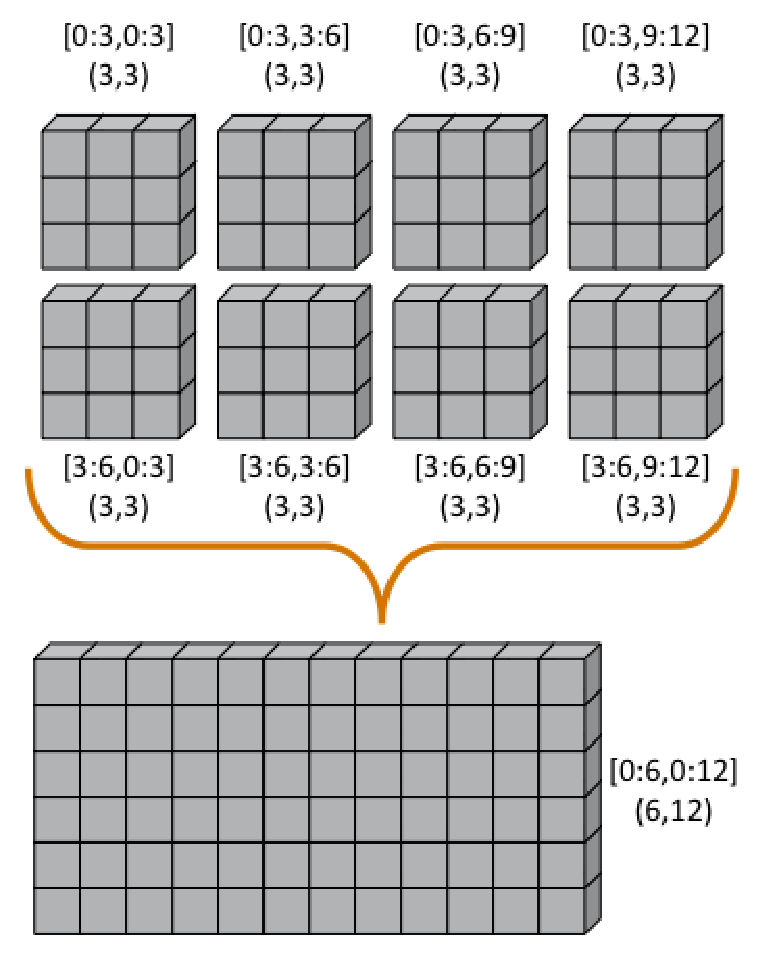
\includegraphics[width=0.47\textwidth]{image1_crop.eps}
\caption{
Each local piece of the gain.ndarray has its own shape (in parenthesis)
and knows its portion of the distribution (in square brackets).  Each local
piece also knows the global shape.
}
\label{fig:1}
\end{figure}

A fundamental design decision was whether to subclass \verb=ndarray= or to
provide a work-alike replacement for the entire \verb=numpy= module. The NumPy
documentation states that \verb=ndarray= implements \verb=__new__()= in order
to control array creation via constructor calls, view casting, and slicing.
Subclasses implement \verb=__new__()= for when the constructor is called
directly, and \linebreak\verb=__array_finalize__()= in order to set additional
attributes or further modify the object from which a view has been taken. One
can imagine an \verb=ndarray= subclass called \verb=gainarray= circumventing
the usual \verb=ndarray= base class memory allocation and instead allocating a
smaller \verb=ndarray= per process while retaining the global \verb=shape=.
One problem occurs with view casting -- with this approach the other
\verb=ndarray= subclasses know nothing of the distributed nature of the memory
within the \verb=gainarray=. NumPy itself is not designed to handle
distributed arrays. By design, ufuncs create an output array when one is not
specified. The first hook which NumPy provides is \verb=__array_prepare__()=
which is called \emph{after the output array has been created}. This means any
ufunc operation on one or more \verb=gainarray= instances without a specified
output would automatically allocate the entire output on each process. For
this reason alone, we opted to reimplement the entire \verb=numpy= module,
controlling all aspects of array creation and manipulation to take into
account distributed arrays.

We present a new Python module, \verb=gain=, developed as part of the main
Global Arrays software distribution. The release of GA v5.0 contained Python
bindings based on the complete GA C API, available in the extension module
\verb=ga=. The GA bindings as well as the \verb=gain= module were developed
using Cython. With the upcoming release of GA v5.1, the module \verb=ga.gain=
is available as a drop-in replacement for NumPy.  The goal of the
implementation is to allow users to write
\begin{minted}[]{python}
import ga.gain as numpy
\end{minted}
and then to execute their code using the MPI process manager
\begin{minted}[]{bash}
mpiexec -np 4 python script.py
\end{minted}

In order to succeed as a drop-in replacement, all attributes, functions,
modules, and classes which exist in \verb=numpy= must also exist within
\verb=gain=.  Efforts were made to reuse as much of \verb=numpy= as possible,
such as its type system. As of GA v5.1, arrays of arbitrary fixed-size element
types and sizes can be created and individual fields of C \verb=struct= data
types accessed directly.  GAiN is able to use the \verb=numpy= types when
creating the GA instances which back the \verb=gain.ndarray= instances. GAiN
is able to use an unmodified NumPy installation and will work with any
sufficiently recent NumPy release.

GAiN follows the owner-computes rule \cite{Zim88}. The rule assigns each
computation to the processor that owns the data being computed. Figures
\ref{fig:2} and \ref{fig:3} illustrate the concept. For any array computation,
GAiN bases the computation on the output array. The processes owning portions
of the output array will acquire the corresponding pieces of the input
array(s) and then perform the computation locally, \emph{calling the original
NumPy routine} on the corresponding array portions. In some cases, for example
if the output array is a view created by a slicing operation, certain
processors will have no computation to perform.

\begin{figure}[htb]
\centering
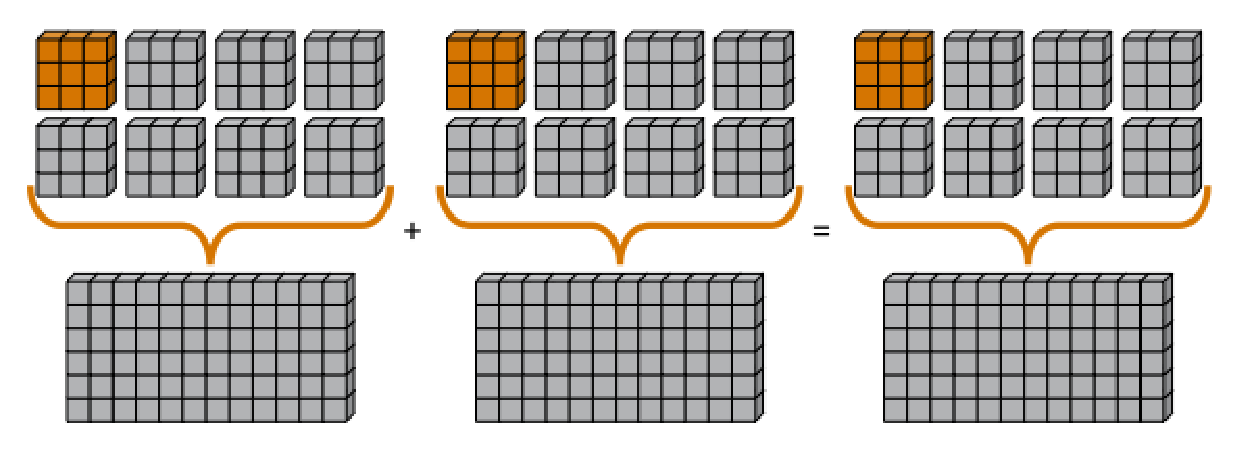
\includegraphics[width=0.47\textwidth]{image3_crop.eps}
\caption{
Add two arrays with the same data distribution. There are eight processors for
this computation.  Following the owner-computes rule, each process owning a
piece of the output array (far right) retrieves the corresponding pieces from
the sliced input arrays (left and middle). For example, the corresponding gold
elements will be computed locally on the owning process.  Note that for this
computation, the data distribution is the same for both input arrays as well
as the output array such that communication can be avoided by using local data
access.
}
\label{fig:2}
\end{figure}

\begin{figure}[htb]
\centering
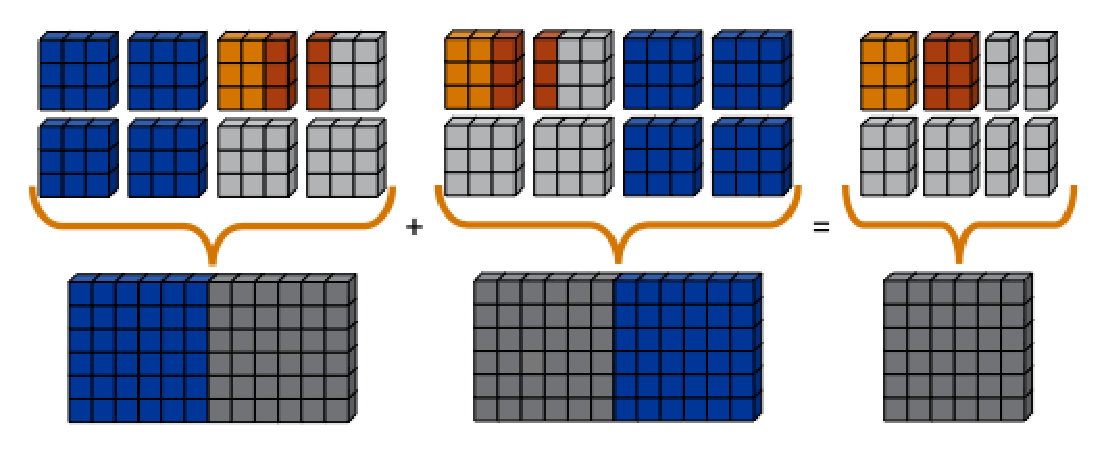
\includegraphics[width=0.47\textwidth]{image2_crop.eps}
\caption{
Add two sliced arrays. There are eight processors for this computation.  The
elements in blue were removed by a slice operation. Following the
owner-computes rule, each process owning a piece of the output array (far
right) retrieves the corresponding pieces from the sliced input arrays (left
and middle). For example, the corresponding gold elements will be computed
locally on the owning process. Similarly for the copper elements.  Note that
for this computation, the data for each array is not equivalently distributed
which will result in communication.
}
\label{fig:3}
\end{figure}

The GAiN implementation of the \verb=ndarray= implements a few important
concepts including the dual nature of a global array and its individual
distributed pieces, slice arithmetic, and separating collective operations
from one-sided operations. When a \verb=gain.ndarray= is created, it creates a
Global Array of the same shape and type and stores the GA integer handle. The
distribution on a given process can be queried using \verb=ga.distribution()=.
The other important attribute of the \verb=gain.ndarray= is the
\verb=global_slice=.  The \verb=global_slice= begins as a list of \verb=slice=
objects based on the original \verb=shape= of the array.

\begin{minted}[]{python}
self.global_slice = [slice(0,x,1) for x in shape]
\end{minted}

Slicing a \verb=gain.ndarray= must return a view just like slicing a
\verb=numpy.ndarray= returns a view. The approach taken is to apply the
\verb=key= of the \verb=__getitem__(key)= request to the \verb=global_slice=
and store the new \verb=global_slice= on the newly created view. We call this
type of operation slice arithmetic. First, the \verb=key= is canonicalized
meaning \verb=Ellipsis= are replaced with \verb=slice(0,dim_max,1)= for each
dimension represented by the \verb=Ellipsis=, all \verb=slice= instances are
replaced with the results of calling \verb=slice.indices()=, and all negative
index values are replaced with their positive equivalents. This step ensures
that the length of the \verb=key= is compatible with and based on the current
shape of the array.  This enables consistent slice arithmetic on the
canonicalized keys. Slice arithmetic effectively produces a new \verb=key=
which, when applied to the same original array, produces the same results had
the same sequence of keys been applied in order. Figures \ref{fig:slice1}
and \ref{fig:figslice2} illustrate this concept.

\begin{figure}[htb]
\centering
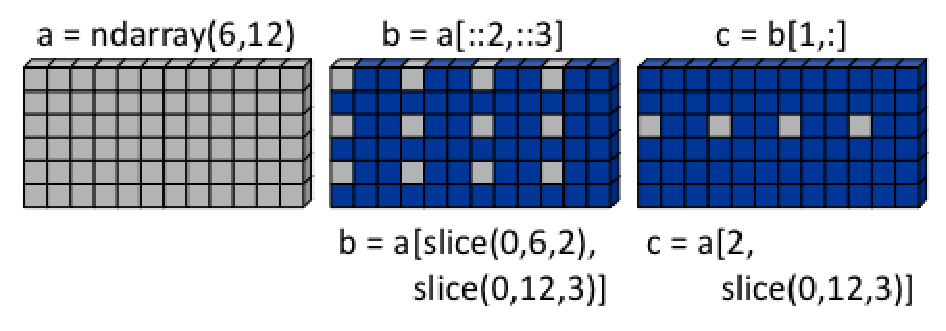
\includegraphics[width=0.47\textwidth]{image4a_crop.eps}
\caption{
Slice arithmetic example 1. Array $b$ could be created either using the
standard notation (top middle) or using the canonicalized form (bottom
middle). Array $c$ could be created by applying the standard notation (top
right) or by applying the equivalent canonical form (bottom right) to the
original array $a$.
}
\label{fig:slice1}
\end{figure}

\begin{figure}[htb]
\centering
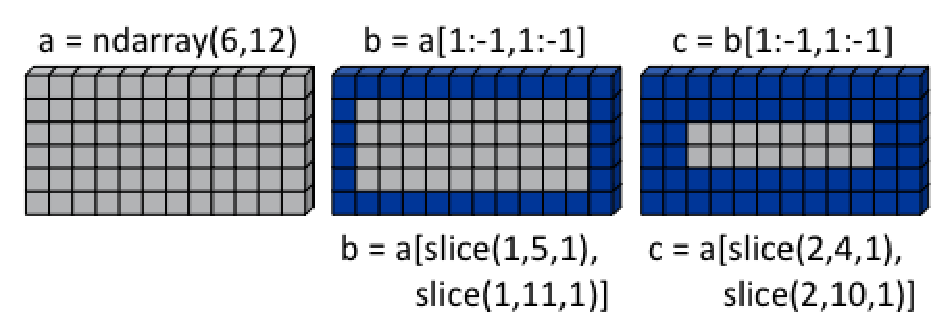
\includegraphics[width=0.47\textwidth]{image4b_crop.eps}
\caption{
Slice arithmetic example 2. See the caption of Figure \ref{fig:slice1} for
details.
}
\label{fig:figslice2}
\end{figure}

When performing calculations on a \verb=gain.ndarray=, the current
\verb=global_slice= is queried when accessing the local data or fetching
remote data such that an appropriate \verb=ndarray= data block is returned.
Accessing local data and fetching remote data is performed by the
\verb=gain.ndarray.access()= and \verb=gain.ndarray.get()= methods,
respectively.  Figure \ref{fig:accessget} illustrates how \verb=access()= and
\verb=get()= are used. The \verb=ga.access()= function on which\linebreak
\verb=gain.ndarray.access()= is based will always return the entire block
owned by the calling process. The returned piece must be further sliced to
appropriately match the current \verb=global_slice=. The
\verb=ga.strided_get()= function on which \verb=gain.ndarray.get()= method is
based will fetch data from other processes without the remote processes'
cooperation i.e. using one-sided communication.  The calling process specifies
the region to fetch based on the current view's \verb=shape= of the array. The
\verb=global_slice= is adjusted to match the requested region using slice
arithmetic and then transformed into a \verb=ga.strided_get()= request based
on the global, original shape of the array.

\begin{figure}[htb]
\centering
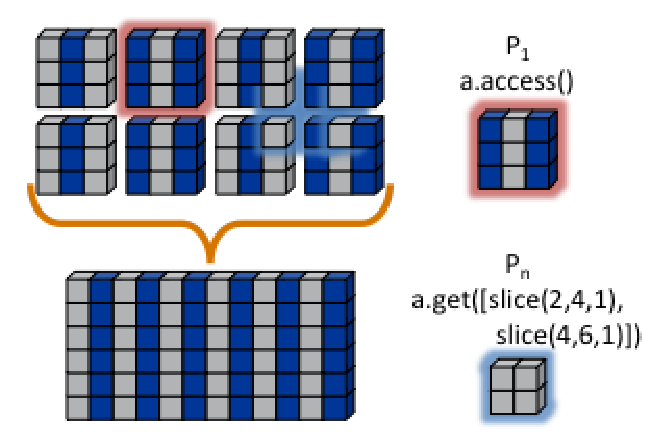
\includegraphics[width=0.47\textwidth]{image5_crop.eps}
\caption{
\texttt{access()} and \texttt{get()} examples. The current
\texttt{global\_slice}, indicated by blue array elements, is respected in
either case. A process can access its local data block for a given array (red
highlight). Note that \texttt{access()} returns the entire block, including
the sliced elements.  Any process can fetch any other processes' data using
\texttt{get()} with respect to the current \texttt{shape} of the array (blue
highlight).  Note that the fetched block will not contain the sliced elements,
reducing the amount of data communicated.
}
\label{fig:accessget}
\end{figure}

Recall that GA allows the contiguous, process-local data to be accessed using
\verb=ga.access()= which returns a C-contiguous \verb=ndarray=. However, if
the \verb=gain.ndarray= is a view created by a slice, the data which is
accessed will be contiguous while the view is not. Based on the distribution
of the process-local data, a new slice object is created from the
\verb=global_slice= and applied to the accessed \verb=ndarray=, effectively
having applied first the \verb=global_slice= on the global representation of
the distributed array followed by a slice representing the process-local
portion.

After process-local data has been accessed and sliced as needed, it must then
fetch the remote data. This is again done using \verb=ga.get()= or
\verb=ga.strided_get()= as above.  Recall that one-sided communication, as
opposed to two-sided communication, does not require the cooperation of the
remote process(es). The local process simply fetches the corresponding array
section by performing a similar transformation to the target array's
\verb=global_slice= as was done to access the local data, and then translates
the modified \verb=global_slice= into the proper arguments for \verb=ga.get()=
if the \verb=global_slice= does not contain any \verb=step= values greater
than one, or \verb=ga.strided_get()= if the \verb=global_slice= contained
\verb=step= values greater than one.

One limitation of using GA is that GA does not allow negative stride values
corresponding to the negative \verb=step= values allowed for Python sequences
and NumPy arrays. Supporting negative \verb=step= values for GAiN required
special care -- when a negative \verb=step= is encountered during a slice
operation, the slice is applied as usual. However, prior to accessing or
fetching data, the slice is inverted from a negative \verb=step= to a positive
\verb=step= and the \verb=start= and \verb=stop= values are updated
appropriately. The \verb=ndarray= which results from accessing or fetching
based on the inverted slice is then re-inverted, creating the correct view of
the new data.

Another limitation of using GA is that the data distribution cannot be changed
once an array is created. This complicates such useful functionality as
\verb=numpy.reshape()=. Currently, GAiN must make a copy of the array instead
of a view when altering the shape of an array.

Translating the \verb=numpy.flatiter= class, which assumes a single address
space while translating an N-dimensional array into a 1D array, into a
distributed form was made simpler by the use of \verb=ga.gather()= and
\verb=ga.scatter()=. These two routines allow individual data elements within
a GA to be fetched or updated.  Flattening a distributed N-dimensional array
which had been distributed in blocked fashion will cause the blocks to become
discontiguous. Figure \ref{fig:flatten} shows how a $6 \times 6$ array
might be distributed and flattened.  The \verb=ga.get()= operation assumes the
requested patch has the same number of dimensions as the array from which the
patch is requested. Reshaping, in general, is made difficult by GA and its
lack of a redistribute capability.  However, in this case, we can use
\verb=ga.gather()= and \verb=ga.scatter()= to fetch and update, respectively,
any array elements in any order.  \verb=ga.gather()= takes a 1D array-like of
indices to fetch and returns a 1D \verb=ndarray= of values. Similarly,
\verb=ga.scatter()= takes a 1D array-like of indices to update and a 1D
array-like buffer containing the values to use for the update. If a
\verb=gain.flatiter= is used as the output of an operation, following the
owner-computes rule is difficult. Instead, pseudo-owners are assigned to
contiguous slices of the of 1D view. These pseudo-owners gather their own
elements as well as the corresponding elements of the other inputs, compute
the result, and scatter the result back to their own elements. This results in
additional communication which is otherwise avoided by true adherence to the
owner-computes rule. To avoid this inefficiency, there are some cases where
operating over \verb=gain.flatiter= instances can be optimized, for example
with \verb=gain.dot()= if the same \verb=flatiter= is passed as both inputs,
the \verb=base= of the \verb=flatiter= is instead multiplied together
element-wise and then the \verb=gain.sum()= is taken of the resulting array.

\begin{figure}[htb]
\centering
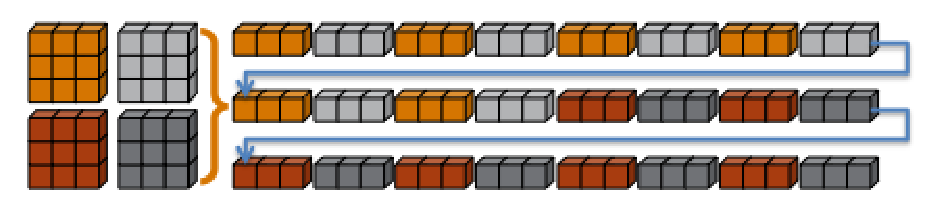
\includegraphics[width=0.47\textwidth]{image6_crop.eps}
\caption{
Flattening a 2D distributed array. The block owned by a process becomes
discontiguous when representing the 2D array in 1 dimension.
}
\label{fig:flatten}
\end{figure}

Not all NumPy programs are suitable for SPMD execution. If the NumPy program
has made assumptions about a single process environment, there must be a
separation between Python running as a single process and a parallel back-end
where the parallel computation is performed. For example, the program might
open a connection to a database. Doing so with multiple processes and in
addition having each process make multiple updates to that database would be
disastrous. Explicit knowledge on the user’s part of the parallel nature of
the execution environment would be needed to mitigate database access.

NumPy programs unsuitable for SPMD execution can be handled by utilizing
master/slave parallelism. The original program assumes the role of master
while any expression involving a \texttt{gain.ndarray} is serialized and sent
to an SPMD parallel back-end. Unless the data being operated on already exists
on the slaves, both the data and the function to operate on the data must be
sent. To accomplish this master/slave parallelism, we use the process
management features of the MPI-2 specification as well as custom Python code
to serialize the objects.

\section{Evaluation}

The success of GAiN hinges on its ability to enable distributed array
processing in NumPy, to transparently enable this processing, and most
importantly to efficiently accomplish those goals. Performance Python
\cite{Ram08} “perfpy” was conceived to demonstrate the ways Python can be used
for high performance computing. It evaluates NumPy and the relative
performance of various Python extensions to NumPy. It represents an important
benchmark by which any additional high performance numerical Python module
should be measured. The original program \verb=laplace.py= was modified by
importing \verb=ga.gain= in place of \verb=numpy= and then stripping the
additional test codes so that only the \verb=gain= (\verb=numpy=) test
remained. The latter modification makes no impact on the timing results since
all tests are run independently but was necessary because \verb=gain= is run
on multiple processes while the original test suite is serial.  The program
was run on the chinook supercomputer at the Environmental Molecular Sciences
Laboratory, part of Pacific Northwest National Laboratory.  Chinook consists
of 2310 HP DL185 nodes with dual socket, 64-bit, Quad-core AMD 2.2 GHz Opteron
processors. Each node has 32 Gbytes of memory for 4 Gbytes per core. Fast
communication between the nodes is obtained using a single rail Infiniband
interconnect from Voltaire (switches) and Melanox (NICs). The system runs a
version of Linux based on Red Hat Linux Advanced Server.  GAiN utilized up to
512 nodes of the cluster, using 4 cores per node.

In Figure \ref{fig:laplace}, GAiN is shown to scale up to 2K cores on a modest
problem size. However, the startup cost of the Python interpreter became
prohibitively large such that a 4K core test could not be run in a reasonable
amount of time. It is encouraging that the implementation of GAiN allows the
algorithm to scale so long as the Python interpreter can be sufficiently
modified to scale, as well.

GAiN is also able to run on problems which are not feasible on workstations.
For example, to store one 100,000x100,000 matrix of double-precision numbers
requires approximately 75GB. 

\begin{figure}[htb]
\centering
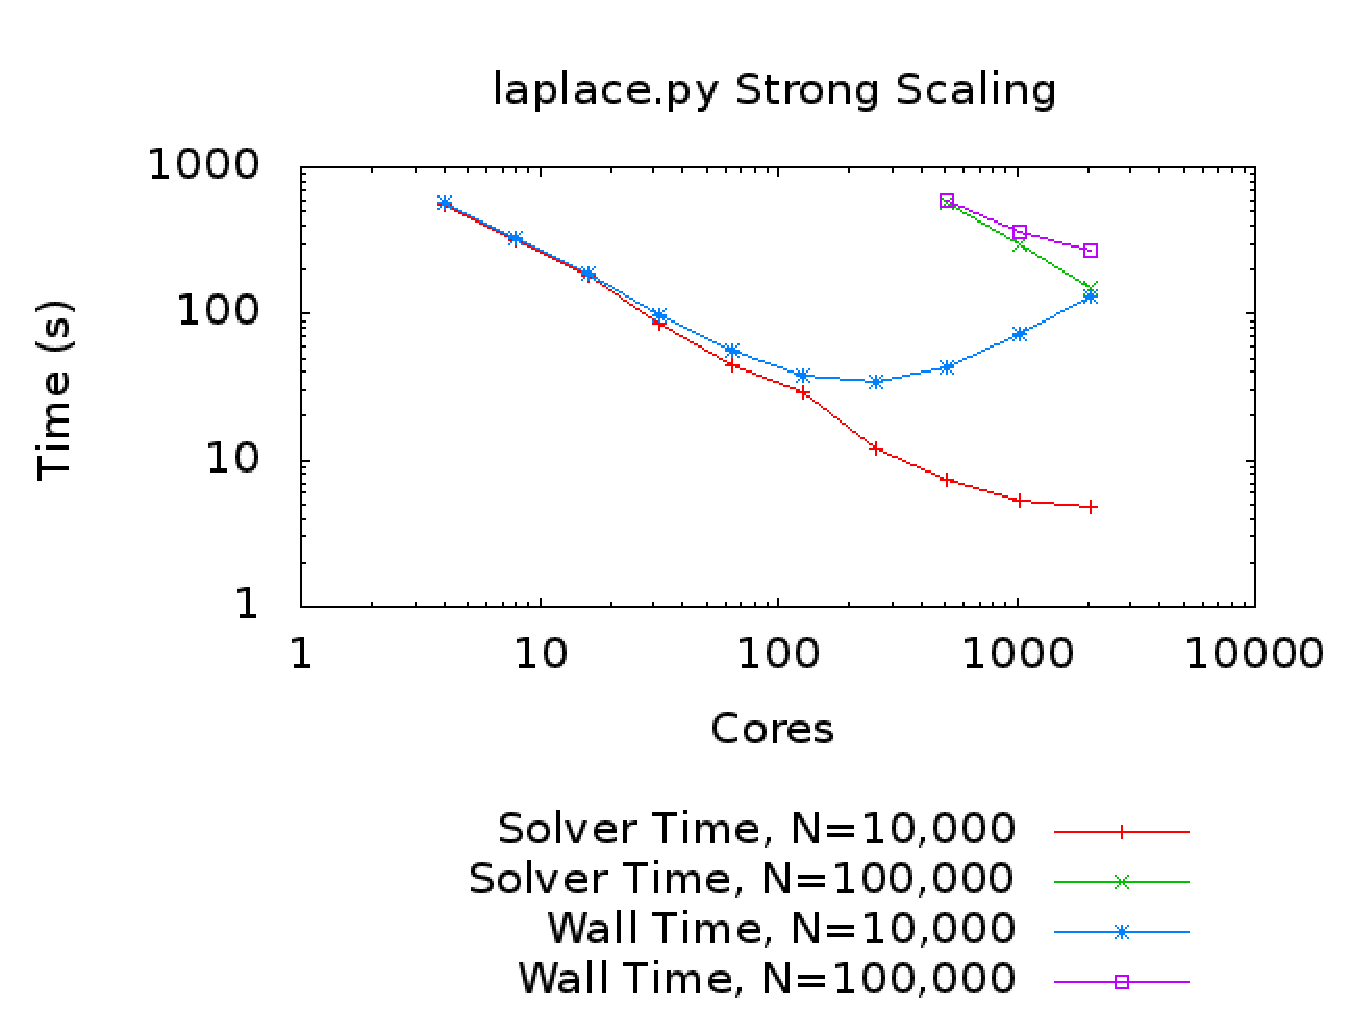
\includegraphics[width=0.47\textwidth]{laplace.eps}
\caption{
\texttt{laplace.py} for N=10,000 and N=100,000. For N=10,000, one matrix
of double-precision numbers is approximately 0.75GB. For this problem, GAiN
scales up to 2K cores in terms of the solver algorithm, however, the Python
interpreter fails to scale beyond a few hundred cores in this case. For
N=100,000, one matrix of double-precision numbers is approximately 75GB. In
addition to handling this large-scale problem, GAiN continues to scale up to
2K cores. Again, the startup cost of the Python interpreter prohibited the 4K
run from starting in a reasonable amount of time.
}
\label{fig:laplace}
\end{figure}

During the evaluation, it was noted that a lot of time was spent within global
synchronization calls e.g. \verb=ga.sync()=. The source of the calls was
traced to, among other places, the vast number of temporary arrays getting
created.  Using GA statistics reporting, the original \verb=laplace.py= code
created 912 arrays and destroyed 910. Given this staggering figure, an array
cache was created. The cache is based on a Python \verb=dict= using the shape
and type of the arrays as the keys and stores discarded GA instances
represented by the GA integer handle. The number of GA handles stored per
shape and type is referred to as the cache depth. The \verb=gain.ndarray=
instances are discarded as usual.  Utilizing the cache keeps the GA memory
from many allocations and deallocations but primarily avoids many
synchronization calls. Three cache depths were tested, as shown in Table
\ref{tab:cache}. The trade-off of using this cache is that if the arrays used
by an application vary wildly in size or type, this cache will consume too
much memory. Other heuristics could be developed to keep the cache from using
too much memory e.g. a maximum size of the cache, remove the least used
arrays, remove the least recently used.  Based on the success of the GA cache,
it is currently used by GAiN.

\begin{table}
\begin{center}
%\begin{tabular}{|l|l|l|}
\begin{tabular}{l|l|l}
%\hline
              & Create & Destroy \\
\hline
No Cache      & 912    & 910     \\
%\hline
Depth-1 Cache & 311    & 306     \\
%\hline
Depth-2 Cache & 110    & 102     \\
%\hline
Depth-3 Cache &  11    &   1     \\
%\hline
\end{tabular}
\caption{
How array caching affects GA array creation/destruction counts when running
\texttt{laplace.py} for 100 iterations. The smaller numbers indicate better
reuse of GA memory and avoidance of global synchronization calls, at the
expense of using additional memory.
}
\label{tab:cache}
\end{center}
\end{table}

\section{Conclusion}

GAiN succeeds in its ability to grow problem sizes beyond a single compute
node. The performance of the perfpy code and the ability to drop-in GAiN
without modification of the core implementation demonstrates its utility. As
described previously, GAiN allows certain classes of existing NumPy programs
to run using GAiN with sometimes as little effort as changing the import
statement, immediately taking advantage of the ability to run in a cluster
environment. Once a smaller-sized program has been developed and tested on a
desktop computer, it can then be run on a cluster with very little effort.
GAiN provides the groundwork for large distributed multidimensional arrays
within NumPy.

\section{Future Work}

GAiN is not a complete implementation of the NumPy API nor does it represent
the only way in which distributed arrays can be achieved for NumPy.
Alternative parallelization strategies besides the owner-computes rule should
be explored. GA allows for the get-compute-put model of computation where
ownership of data is largely ignored while data movement costs are increased.
However, the get-compute-put model of computation may allow an algorithm to
mix communication and computation, improving overall performance as is done
with the SRUMMA dense matrix multiplication algorithm \cite{Kri04}.

Task parallelism could also be explored if load balancing becomes an issue.
The scioto framework \cite{Din08} interoperates with MPI and GA and provides
locality-aware dynamic load balancing via management of shared collections of
task objects. Certain NumPy functionality may better lend itself to task
parallelism instead of owner-computes. Task parallelism decouples data
ownership from the computation and is more akin to the get-compute-put model.
Further, GAiN does not support block cyclic data distributions. Block cyclic
distributions may alleviate load imbalance but may also incur additional
overhead.

The GA cache should be exposed as a tunable parameter since the current
heuristic of reusing arrays with the same type and shape does not apply to
dynamic applications. For example, while not a true application, the current
test suite for GAiN creates many arrays of different shapes and types. Most of
those arrays are not reused. Applications of this nature may wish to disable
GA caching.  Alternative temporary array creation strategies and heuristics
could also be developed.

Although the GA cache is meant to solve the problem of temporary array
creation which occurs through normal use of the NumPy API,  it does not solve
the problem of combining arithmetic operations. Packages such as
\emph{numexpr} \cite{Coo11} and \emph{Metagraph} \cite{Wan11} evaluate
multiple-operator NumPy expressions many times faster than NumPy. numexpr
works by combining arithmetic operations, reducing temporary array creation,
and utilizing vectorizing libraries. A similar approach could be utilized by
GAiN. The approach taken by numexpr is similar to the approach used by GpuPy
discussed earlier. GpuPy utilizes lazy evaluation to store NumPy functions as
an abstract syntax tree to combine arithmetic operations on a GPU.

Although the master/slave capabilities of GAiN allow for most NumPy
applications to parallelize their NumPy portions alone, utilizing the MPI-2
specification may not be the preferred approach. The distributed computing
capabilities of the IPython project may provide another means of separating
the serial from the parallel. The approach taken by DistNumPy does not
involve MPI-2 dynamic process management but rather has all processes besides
the master process block for task messages during the module import. There may
be other ways to separate the serial from the parallel which don't involve
dynamic process management such as processor groups or careful use of
branching within the code effectively emulating a master/slave situation like
DistNumPy.

The scalability of the Python interpreter remains an open problem. This is the
single greatest hurdle to running Python applications at scale. There is a
potential solution for diskless systems such as BlueGene/P machines provided
by \cite{Scu11}. Clusters with local disks mounted to their compute nodes may
find other approaches valuable, as well.

%\appendix
%\section{Appendix Title}
%
%This is the text of the appendix, if you need one.

\acks

A portion of the research was performed using the Molecular Science Computing
(MSC) capability at EMSL, a national scientific user facility sponsored by the
Department of Energy’s Office of Biological and Environmental Research and
located at Pacific Northwest National Laboratory (PNNL). PNNL is operated by
Battelle for the U.S. Department of Energy under contract DE-AC05-76RL01830.

% We recommend abbrvnat bibliography style.

%\bibliographystyle{abbrvnat}
%\bibliography{bibliography}

\begin{thebibliography}{36}
\providecommand{\natexlab}[1]{#1}
\providecommand{\url}[1]{\texttt{#1}}
\expandafter\ifx\csname urlstyle\endcsname\relax
  \providecommand{\doi}[1]{doi: #1}\else
  \providecommand{\doi}{doi: \begingroup \urlstyle{rm}\Url}\fi

\bibitem[Pnl(2011)]{Pnl11}
Global arrays webpage.
\newblock http://www.emsl.pnl.gov/docs/global/, 2011.

\bibitem[Apr\'{a} et~al.(2009)Apr\'{a}, Rendell, Harrison, Tipparaju, deJong,
  and Xantheas]{Apr09}
E.~Apr\'{a}, A.~P. Rendell, R.~J. Harrison, V.~Tipparaju, W.~A. deJong, and
  S.~S. Xantheas.
\newblock Liquid water: obtaining the right answer for the right reasons.
\newblock In \emph{SC}. ACM, 2009.
\newblock ISBN 978-1-60558-744-8.

\bibitem[Ascher et~al.(1999)Ascher, Dubois, Hinsen, Hugunin, , and
  Oliphant]{Asc99}
D.~Ascher, P.~F. Dubois, K.~Hinsen, J.~Hugunin, , and T.~Oliphant.
\newblock Numerical python.
\newblock Technical Report UCRL-MA-128569, Lawrence Livermore National
  Laboratory, 1999.

\bibitem[Behnel et~al.(2011)Behnel, Bradshaw, Citro, Dalcin, Seljebotn, and
  Smith]{Beh11}
S.~Behnel, R.~Bradshaw, C.~Citro, L.~Dalcin, D.~S. Seljebotn, and K.~Smith.
\newblock Cython: The best of both worlds.
\newblock \emph{Computing in Science Engineering}, 13\penalty0 (2):\penalty0
  31--39, 2011.

\bibitem[Buyya(1999)]{Buy99}
R.~Buyya.
\newblock \emph{High Performance Cluster Computing: Architectures and Systems}.
\newblock Prentice Hall PTR, Upper Saddle River, NJ, USA, 1999.
\newblock ISBN 0130137847.

\bibitem[Cooke and Hochberg()]{Coo11}
D.~Cooke and T.~Hochberg.
\newblock numexpr.
\newblock http://code.google.com/p/numexpr/.

\bibitem[Daily(2009)]{Dai09}
J.~Daily.
\newblock Gain: Distributed array computation with python.
\newblock Technical Report PNNL-18355, Pacific Northwest National Laboratory,
  2009.

\bibitem[Daily and Lewis(2011)]{Dai11}
J.~Daily and R.~R. Lewis.
\newblock Using the global arrays toolkit to reimplement numpy for distributed
  computation.
\newblock In \emph{Proceedings of the 10th Python in Science Conference}, 2011.

\bibitem[Dalc\'{\i}n et~al.(2005)Dalc\'{\i}n, Paz, and Storti]{Dal05}
L.~Dalc\'{\i}n, R.~Paz, and M.~Storti.
\newblock Mpi for python.
\newblock \emph{J. Parallel Distrib. Comput.}, 65:\penalty0 1108--1115,
  September 2005.
\newblock ISSN 0743-7315.
\newblock \doi{http://dx.doi.org/10.1016/j.jpdc.2005.03.010}.

\bibitem[Dalc\'{\i}n et~al.(2008)Dalc\'{\i}n, Paz, Storti, and
  D'El\'{\i}a]{Dal08}
L.~Dalc\'{\i}n, R.~Paz, M.~Storti, and J.~D'El\'{\i}a.
\newblock Mpi for python: Performance improvements and mpi-2 extensions.
\newblock \emph{J. Parallel Distrib. Comput.}, 68:\penalty0 655--662, May 2008.
\newblock ISSN 0743-7315.
\newblock \doi{10.1016/j.jpdc.2007.09.005}.

\bibitem[Dinan et~al.(2008)Dinan, Krishnamoorthy, Larkins, Nieplocha, and
  Sadayappan]{Din08}
J.~Dinan, S.~Krishnamoorthy, D.~B. Larkins, J.~Nieplocha, and P.~Sadayappan.
\newblock Scioto: A framework for global-view task parallelism.
\newblock In \emph{ICPP}, pages 586--593. IEEE Computer Society, 2008.

\bibitem[Dotsenko et~al.(2004)Dotsenko, Coarfa, and Mellor-Crummey]{Dot04}
Y.~Dotsenko, C.~Coarfa, and J.~Mellor-Crummey.
\newblock A multi-platform co-array fortran compiler.
\newblock In \emph{Proceedings of the 13th International Conference on Parallel
  Architectures and Compilation Techniques}, PACT '04, pages 29--40,
  Washington, DC, USA, 2004. IEEE Computer Society.
\newblock ISBN 0-7695-2229-7.
\newblock \doi{http://dx.doi.org/10.1109/PACT.2004.3}.

\bibitem[Dubois et~al.(1996)Dubois, Hinsen, and Hugunin]{Dub96}
P.~F. Dubois, K.~Hinsen, and J.~Hugunin.
\newblock Numerical python.
\newblock \emph{Computers in Physics}, 10, May/June 1996.

\bibitem[Edelman(2007)]{Ede07}
A.~Edelman.
\newblock The star-p high performance computing platform.
\newblock In \emph{Acoustics, Speech and Signal Processing, 2007. ICASSP 2007.
  IEEE International Conference on}, volume~4, pages IV--1197 --IV--1200, april
  2007.
\newblock \doi{10.1109/ICASSP.2007.367290}.

\bibitem[Eitzen(2007)]{Eit07}
B.~Eitzen.
\newblock Gpupy: Efficiently using a gpu with python.
\newblock Master's thesis, Washington State University, 2007.

\bibitem[Gropp et~al.(1999{\natexlab{a}})Gropp, Lusk, and Skjellum]{Gro99a}
W.~Gropp, E.~Lusk, and A.~Skjellum.
\newblock \emph{Using MPI: Portable Parallel Programming with the
  Message-Passing Interface}.
\newblock MIT Press, 2 edition, November 1999{\natexlab{a}}.
\newblock ISBN 978-0-262-57132-6.

\bibitem[Gropp et~al.(1999{\natexlab{b}})Gropp, Lusk, and Thakur]{Gro99b}
W.~Gropp, E.~Lusk, and R.~Thakur.
\newblock \emph{Using MPI-2: Advanced Features of the Message-Passing
  Interface}.
\newblock MIT Press, November 1999{\natexlab{b}}.
\newblock ISBN 978-0-262-57133-3.

\bibitem[Harrison(1999)]{Har99}
R.~J. Harrison.
\newblock Global arrays python interface.
\newblock http://www.emsl.pnl.gov/docs/global/old/pyGA, December 1999.

\bibitem[Husbands and Isbell(1999)]{Hus98}
P.~Husbands and C.~Isbell.
\newblock The parallel problems server: A client-server model for interactive
  large scale scientific computation.
\newblock In \emph{Selected Papers and Invited Talks from the Third
  International Conference on Vector and Parallel Processing}, VECPAR '98,
  pages 156--169, London, UK, 1999. Springer-Verlag.
\newblock ISBN 3-540-66228-6.

\vfill\eject

\bibitem[III(2007)]{Pal07}
W.~P. III.
\newblock \emph{A Concise Introduction to Matlab}.
\newblock McGraw-Hill Science/Engineering/Math, October 2007.
\newblock ISBN 978-0073385839.

\bibitem[Krishnan and Nieplocha(2004)]{Kri04}
M.~Krishnan and J.~Nieplocha.
\newblock Srumma: a matrix multiplication algorithm suitable for clusters and
  scalable shared memory systems.
\newblock In \emph{in proceedings of Parallel and Distributed Processing
  Symposium}, 2004.

\bibitem[Kristensen and Vinter(2010)]{Kri10}
M.~R.~B. Kristensen and B.~Vinter.
\newblock {Numerical Python for Scalable Architectures}.
\newblock In \emph{Fourth Conference on Partitioned Global Address Space
  Programming Model, PGAS{'}10}. ACM, 2010.

\bibitem[Lundh(2001)]{Lun01}
F.~Lundh.
\newblock \emph{Python Standard Library}.
\newblock O'Reilly Media, May 2001.
\newblock ISBN 978-0-596-00096-7.

\bibitem[Nieplocha et~al.(2000)Nieplocha, Ju, and Straatsma]{Nie00}
J.~Nieplocha, J.~Ju, and T.~P. Straatsma.
\newblock A multiprotocol communication support for the global address space
  programming model on the ibm sp.
\newblock In \emph{Proceedings from the 6th International Euro-Par Conference
  on Parallel Processing}, Euro-Par '00, pages 718--728, London, UK, 2000.
  Springer-Verlag.
\newblock ISBN 3-540-67956-1.
\newblock URL \url{http://portal.acm.org/citation.cfm?id=646665.699092}.

\bibitem[Nieplocha et~al.(2005{\natexlab{a}})Nieplocha, Krishnan, Palmer,
  Tipparaju, and Zhang]{Nie05}
J.~Nieplocha, M.~Krishnan, B.~Palmer, V.~Tipparaju, and Y.~Zhang.
\newblock Exploiting processor groups to extend scalability of the ga shared
  memory programming model.
\newblock In \emph{Proceedings of the 2nd conference on Computing frontiers},
  CF '05, pages 262--272, New York, NY, USA, 2005{\natexlab{a}}. ACM.
\newblock ISBN 1-59593-019-1.
\newblock \doi{http://doi.acm.org/10.1145/1062261.1062305}.
\newblock URL \url{http://doi.acm.org/10.1145/1062261.1062305}.

\bibitem[Nieplocha et~al.(2005{\natexlab{b}})Nieplocha, Palmer, Krishnan,
  Trease, and Apr\'{a}]{Nie06}
J.~Nieplocha, B.~Palmer, M.~Krishnan, H.~Trease, and E.~Apr\'{a}.
\newblock Advances, applications and performance of the global arrays shared
  memory programming toolkit.
\newblock \emph{Intern. J. High Perf. Comp. Applications}, 20,
  2005{\natexlab{b}}.

\bibitem[Nieplocha et~al.(2010)Nieplocha, Krishnan, Palmer, Tipparaju, and
  Ju]{Nie10}
J.~Nieplocha, M.~Krishnan, B.~Palmer, V.~Tipparaju, and J.~Ju.
\newblock The gobal arrays user's manual.
\newblock http://www.emsl.pnl.gov/docs/global/um/UG-PDF/GA-UserManual-Main.pdf,
  2010.

\bibitem[Oliphant(2006)]{Oli06}
T.~E. Oliphant.
\newblock Guide to numpy.
\newblock http://www.tramy.us/, 2006.

\bibitem[Panuganti et~al.(2006)Panuganti, Baskaran, Hudak, Krishnamurthy,
  Nieplocha, Rountev, , and Sadayappan]{Pan06}
R.~Panuganti, M.~M. Baskaran, D.~E. Hudak, A.~Krishnamurthy, J.~Nieplocha,
  A.~Rountev, , and P.~Sadayappan.
\newblock Gamma: Global arrays meets matlab.
\newblock Technical Report OSU-CISRC-1/06-TR15, Ohio State University, 2006.

\bibitem[Perez et~al.(2009)Perez, Langtangen, and LeVeque]{Per09}
F.~Perez, H.~P. Langtangen, and R.~LeVeque.
\newblock {CSE 2009: Python for Scientific Computing at CSE 2009}.
\newblock SIAM News, 2009.
\newblock URL \url{http://www.siam.org/news/news.php?id=1595}.

\bibitem[P\i{e}rez and Granger(2007)]{Per07}
F.~P\i{e}rez and B.~E. Granger.
\newblock Ipython: A system for interactive scientific computing.
\newblock \emph{Computing in Science and Engineering}, 9:\penalty0 21--29,
  2007.
\newblock ISSN 1521-9615.
\newblock \doi{http://doi.ieeecomputersociety.org/10.1109/MCSE.2007.53}.

\bibitem[Ramachandran(2008)]{Ram08}
P.~Ramachandran.
\newblock Performance python.
\newblock http://www.scipy.org/PerformancePython, May 2008.

\bibitem[Rasmussen et~al.(2004)Rasmussen, Sottile, Nieplocha, Numrich, and
  Jones]{Ras04}
C.~E. Rasmussen, M.~J. Sottile, J.~Nieplocha, R.~W. Numrich, and E.~Jones.
\newblock Co-array python: A parallel extension to the python language.
\newblock In \emph{Euro-Par 2004}, pages 632--637. Springer-Verlag Berlin
  Heidelberg, 2004.

\bibitem[Scullin and Ahmadia()]{Scu11}
W.~Scullin and A.~Ahmadia.
\newblock walla.
\newblock https://bitbucket.org/wscullin/walla/overview.

\bibitem[Wang(2011)]{Wan11}
P.~Wang.
\newblock Metagraph: A declarative graphing system for python.
\newblock In \emph{Proceedings of the 10th Python in Science Conference}.
  SciPy, 2011.
\newblock To appear.

\bibitem[Zima et~al.(1988)Zima, Bast, and Gerndt]{Zim88}
H.~P. Zima, H.-J. Bast, and M.~Gerndt.
\newblock Superb: A tool for semi-automatic mimd/simd parallelization.
\newblock \emph{Parallel Computing}, 6:\penalty0 1--18, 1988.
\newblock \doi{10.1016/0167-8191(88)90002-6}.

\end{thebibliography}
% The bibliography should be embedded for final submission.

\end{document}
